\documentclass[12pt]{article}

\usepackage[pdftex]{graphicx} 
\usepackage{amsmath}

\textwidth = 6.5 in
\textheight = 9 in
\oddsidemargin = 0.0 in
\evensidemargin = 0.0 in
\topmargin = 0.0 in
\headheight = 0.0 in
\headsep = 0.0 in
%\parskip = 0.2in
\parskip 6pt
\parindent = 0.0in

%\textwidth 6.5in
%\textheight 9in
%\oddsidemargin 0pt
%\evensidemargin 0pt
%\topmargin -.5in
%\headheight .25in

\newtheorem{theorem}{Theorem}
\newtheorem{corollary}[theorem]{Corollary}
\newtheorem{definition}{Definition}
%% Add next two lines for Adobe type fonts! 12/5/01 Tony Seibert
\fontfamily{ptm}\selectfont
\renewcommand{\rmdefault}{ptm}

%\title{Brief Article}
%\author{The Author}
\begin{document}

%\ifpdf
%\DeclareGraphicsExtensions{.pdf, .jpg, .tif}
%\else
%\DeclareGraphicsExtensions{.eps, .jpg}
%\fi

\DeclareGraphicsExtensions{.pdf, .jpg, .tif}



\begin{center}
\section*{Lab 5: Schmitt Trigger and Relaxation Oscillator}
UC Davis Physics 116B\\
Rev 1/11/2019\\
%%%% Based on Lab14_00}
\end{center}

\section*{Introduction}

\begin{figure}[!h]
\centerline{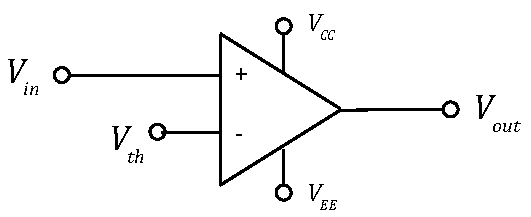
\includegraphics[width=3in]{figs/comparator.pdf}}
\caption{An open loop op-amp as a comparator}
\label{fig:comparator}
\end{figure}

An open loop op-amp can be thought of as a comparator, as shown in Figure~\ref{fig:comparator}, with the following behavior:

\begin{align*}
V_{in}>V_{th} & \rightarrow V_{out}=V_{CC}\\
V_{in}<V_{th}& \rightarrow V_{out}=V_{EE}
\end{align*}

As we discussed in class, this circuit can be unstable for inputs near the threshold.

A Schmitt Trigger uses feedback to change the threshold depending on the output state, in order to
improve its stability.

\section*{Schmitt Trigger}

\begin{figure}[!h]
\centerline{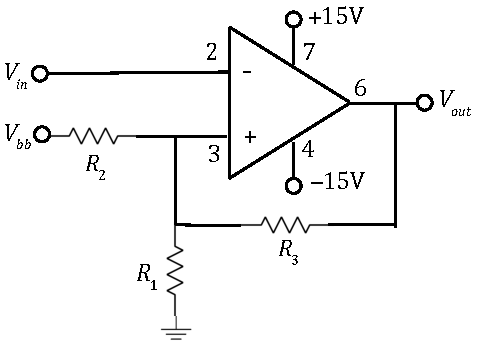
\includegraphics[width=3in]{figs/schmitt.pdf}}
\caption{A Schmitt Trigger}
\label{fig:schmitt}
\end{figure}

The Schmitt trigger circuit is shown in Figure~\ref{fig:schmitt}. Build this circuit using an LM741, with $\pm 15$V power supplies. Use $R_1=R_2=$10k$\Omega$, and $R_3$=100k$\Omega$.  Drive the circuit with a 1kHz triangle wave, with a 20V peak-to-peak amplitude.  Verify the transition threshold
for both the rising and filling slopes and verify that they match the prediction of:
\begin{align*}
V_{th}=\frac{R_1||R_2||R_3}{R_2}V_{bb}+\frac{R_1||R_2||R_3}{R_3}V_{out}
\end{align*}

For your lab report, include images of the scope traces, including a close up on both the rising and falling transition.

\section*{Simulated Noisy Source}

\begin{figure}[!h]
\centerline{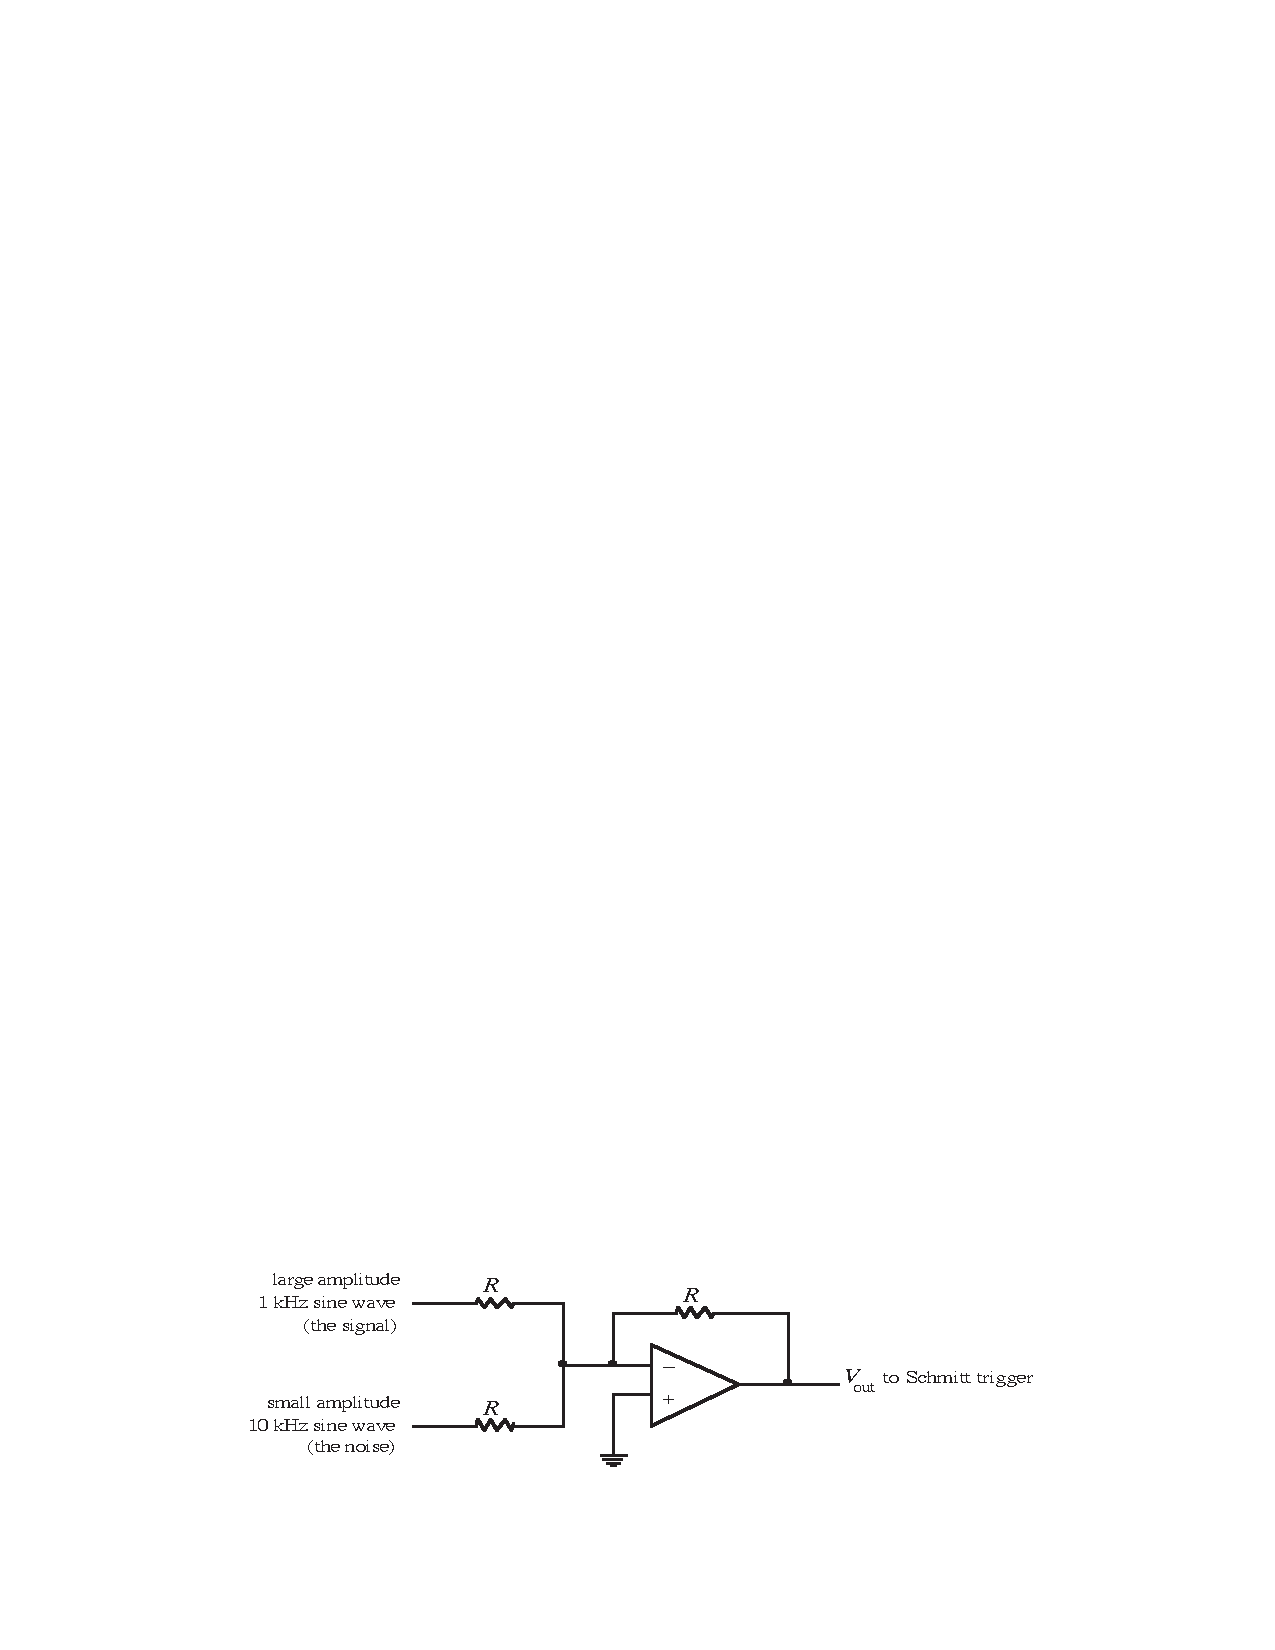
\includegraphics[width=6in]{figs/noisy-signal.pdf}}
\caption{A simulated noise source.}
\label{fig:noisy-signal}
\end{figure}

To see how a Schmitt trigger might be useful, we will construct a source with some fake noise introduced into it. Figure~\ref{fig:noisy-signal} shows how to do this using two function generators and a second 741 op-amp, used as a summing amplifier. Build this circuit and use it as the input to your Schmitt trigger. Make all resistors equal, with values of a few k$\Omega$.  Regard the 1kHz sign wave as the ``signal" and the 10 kHz sine wave as the ``noise". For your lab report, include a picture of the scope trace showing
both the input and the outpu, being careful to show each time the input crosses a Vth and what the output does in response. Determine the amplitude of the ``noise" signal that will cause multiple transitions on the rising edge of the signal.  Include an image of this in your report. 
\section*{Relaxation Oscillator}

\begin{figure}[h!]
\centerline{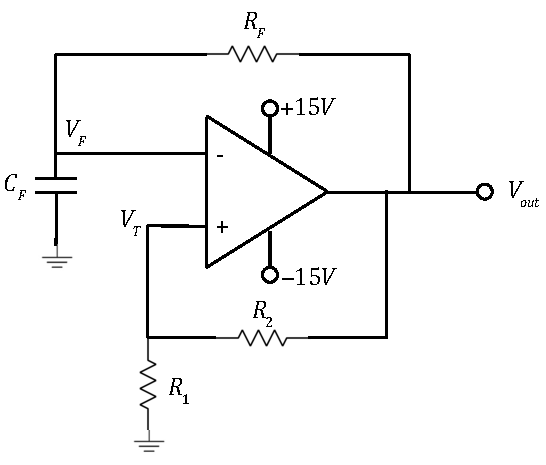
\includegraphics[width=3in]{figs/relaxation.pdf}}
\caption{Relaxation oscillator.}
\label{fig:relaxation}
\end{figure}

Construct the relaxation oscillator shown in Figure~\ref{fig:relaxation}.  Use $R_1=R_2=R_F=10$k$\Omega$ and $C_F$=10nF.  Verify that
the period of the oscillation is
\begin{align*}
T=2R_FC_F\ln\left(\frac{2R_1+R_2}{R_2}\right)
\end{align*}
as we derived in class.

For your lab report, include a picture of the output waveform.


\end{document}



